\section{Related Work}

Dialog systems can be broadly divided into two categories: open domain \cite{vinyals2015neural,serban2016building} and task-oriented dialog systems. Open domain systems generate responses based on just the dialog history, whereas the task-oriented systems generate responses based on the dialog history and a KB associated with the task. 

Task oriented dialogs systems can be further divided into two: modular and end-to-end trainable dialog systems. Modular dialog systems \cite{wen2017network,williams2017hybrid,williams2007partially} require intermediate supervision on dialog transcripts to train each of its modules. Our work falls under end-to-end trainable dialog systems, which requires just the dialog transcripts and no intermediate supervision to train. We discuss end-to-end trainable neural models along two dimensions: (1) decoding: how the response is retrieved or generated and (2) encoding: how the dialog context (dialog history and KB tuples) are represented. 

Most of the existing approaches \cite{BordesW16,liu2017gated,seo2016query,wu2017end} {\em retrieve} a response from a pre-defined set. These methods are generally successful when they have to provide boilerplate responses -- they cannot construct new responses or use words not seen during training. 
To improve upon these, generative approaches are used where the next response is {\em generated} one word at a time \cite{eric2017copy,mem2seq}. These approaches also benefit the OOV problem by incorporating the ability to copy words from the input \cite{vinyals2015pointer,gu2016incorporating}. This copy mechanism has also found success in summarization \cite{nallapati2016abstractive,see2017get} and machine translation \cite{ptr-unk}. \sys\ is a copy incorporated generative approach.

%The dialog context consists of utterances in the past and KB tuples. 
% For encoding, existing approaches either represent the dialog context as {\em set of sets} \cite{mem2seq,BordesW16,liu2017gated} or {\em sequence of sequences} \cite{eric2017copy,ptr-unk}. {\em Set of sets} represents past utterances as a bag of words making it difficult to capture context and work with words not seen during training. {\em Seq of seqs} enforces an order over the set of KB tuples making it harder to perform inferencing over multiple KB tuples. \sys\ uses a {\em set of seqs} representation, which can both capture word contexts and perform inferencing over KB tuples.

For encoding, some approaches represent the dialog history as a sequence \cite{eric2017copy,ptr-unk}. Unfortunately, using a single long sequence for encoding also enforces an order over the set of KB tuples making it harder to perform inferencing over them. Other approaches represent the dialog context as a bag. Original Memory Networks \cite{BordesW16} and its extensions encode each memory element (utterance) as an average of all constituent words -- this cannot point to individual words, and hence cannot be used with a copy mechanism. Mem2Seq encodes each word individually in a flat memory. Unfortunately, this loses the contextual information around a word, which is needed to decipher an unseen word. In contrast, \sys\ uses a bag of sequences encoding, where KB tuples are a set for easier inference, and also each utterance is a sequence for effectively learning when to copy. We go into further detail below highlighting the differences between the two models.


%Attention over hierarchical representation of sentences and words has been used in document classification \cite{yang2016hierarchical} and abstractive text summarization \cite{nallapati2016abstractive}. These representations defines the document as a sequence of sentences while we propose a set to better represent KB tuples.

\subsection{Comparison with Mem2Seq}
\label{sec:relatedmem2seq}
The closest to our model is the recently introduced Mem2Seq \cite{mem2seq}, which also combines the multi-hop reasoning of memory networks with the generative decoding augmented with a copy mechanism. While similar in spirit to \sys, there are significant differences in the two architectures. We illustrate these with Figure \ref{fig:intro}, which shows an example dialog along with an associated KB in both Mem2Seq and \sys\ memories. %Figure \ref{fig:intro}b shows how the dialog is represented in the Mem2Seq memory.

First, the memory in Mem2Seq is a flat representation which operates in part at utterance level and in part at word level. In particular, the individual words of a user/machine utterance are stored in their own memory cells, whereas a KB tuple gets only one memory cell -- the aggregation is done in a bag of words fashion, using words in the entire tuple. For example, the memory element \textit{m1} contains a full KB tuple and \textit{m15} contains only the word ``french'' from the second user utterance.

This implies that Mem2Seq's copy mechanism can only point to a specific KB tuple, but cannot point to a specific constituent of the tuple. This forces Mem2Seq to make a second modeling choice, of allowing only the ``object'' entity of a tuple to be used in the next response. These choices result in three limitations of Mem2Seq, regarding the scenarios in which Mem2Seq can be useful. 


\begin{figure}[t]
\centering
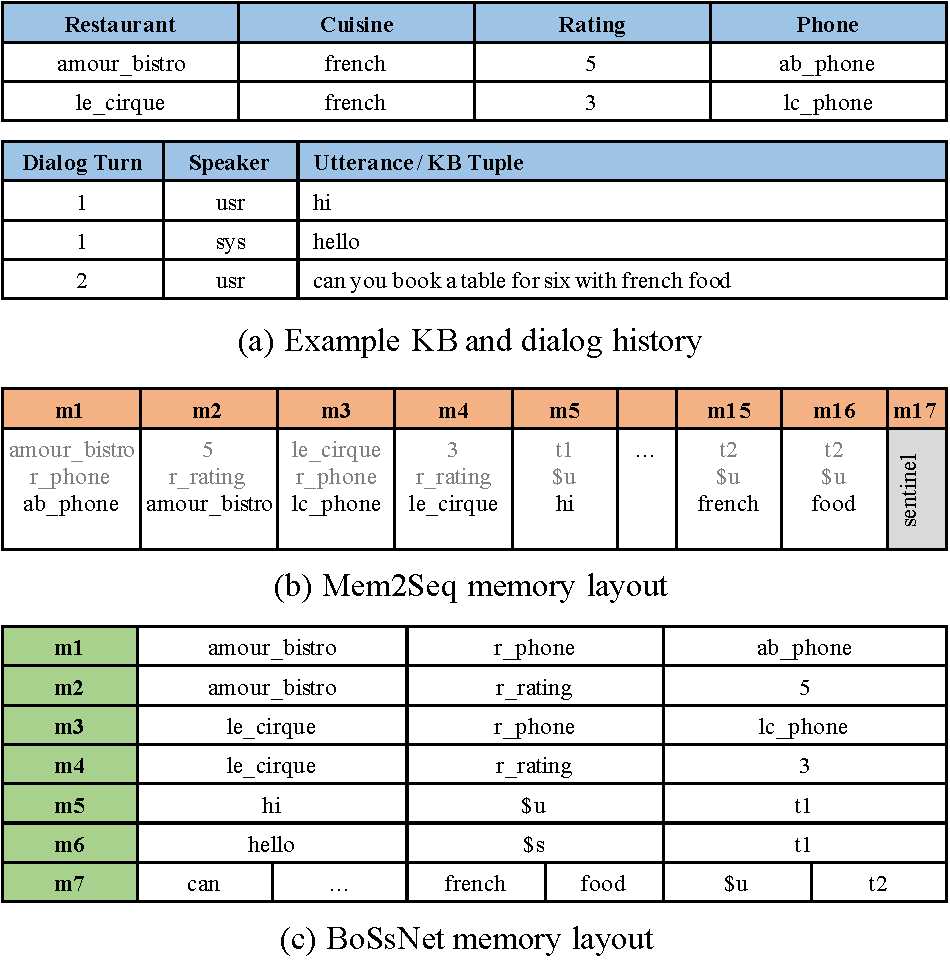
\includegraphics[scale=0.8]{assets/figures/mem2seq.pdf}
\caption{(a) an example dialog with history and KB tuples. (b) an illustration of Mem2Seq memory. (c) an illustration of \sys\ memory}
\label{fig:intro}
\end{figure}

%Our model has the following differences when compared to Mem2Seq: 1) The memory in Mem2Seq has a flat representation whereas we propose a hierarchical representation. 2) The performance of Mem2Seq is dependent on the ordering of KB tuples (subject or object), while the performance of \sys\ is independent of any such ordering. 

% Describe the memory layout
% Each memory element contains either a KB tuple or a word from an utterance in the dialog history. For example, 

% Describe problem #1 and #2
First, Mem2Seq expects each tuple to be serialized by the KB API in way that the object always comes last. This may or may not always be in control of the neural model. Second, because each utterance word has a unique memory cell. it loses the context in which the word was mentioned. As a result, the model cannot learn that ``french'' and other cuisines are usually followed by the word ``food''. This causes poor generalization where the model has to understand an OOV word from the user utterance (e.g., a new cuisine or city name). 
% The vector representation of each memory element is computed using a bag-of-words model. Thus the memory structure prevents the model to generalize by learning clues from the context. 

% Describe problem #3
Finally, the model design dictates that the subject or the predicate from a KB fact can never be copied during the decode step. This adds severe limitations in practical settings. For example, the KB results in the original bAbI dataset \cite{BordesW16} came in format of {\em attribute(restaurant\_name, restaurant\_attribute)}. Since restaurant name is never an object, Mem2Seq would never be able to copy it when making recommendations. As a result, experiments with Mem2Seq necessitated a training data preprocessing, in which all rating facts had to be inverted into {\em rating(restaurant\_rating, restaurant\_name)}, so that the name could become an object and could be copied. 

We believe that this adds severe limitations on the scenarios in which Mem2Seq is applicable. We perform several experiments on the original (unprocessed) datasets to highlight the loss in performance due to these modeling choices. 
In contrast, \sys\ uses a hierarchical memory that can copy {\em any} word from the whole dialog history (see Figure \ref{fig:intro}(c)). It models each cell as a {\em sequence} of words, which also enables it to learn contextual cues for each word, leading to better OOV generalization. 

%The designer needs to carefully choose how a tuple should be placed in the memory. In the example, the object of \textit{r\_phone} (placed at the bottom) is chosen to be the word to copy, while the subject is chosen for \textit{r\_rating}. The placement is dictated by what needs to be copied while generating the response. In the experiments, how ordering affects its performance.

%In the dialog bAbI dataset \cite{BordesW16}, the name of the restaurant and the phone numbers are needed to be copied. Mem2Seq will not be able to generate a response such as ``amour_bistro has a rating of 5'' as the rating object is not addressable by the copy mechanism. 

%Also, if a word occurs more than once in the memory, only the last occurrence of the word is used for computing the copy distribution. This makes the system depend on the order in which KB tuples are placed in the memory
%\todo{Does it fit better now ?}

\section{Components Survey}

\sys\ architecture has a {\em multi-hop encoder}, and a {\em pointer network} decoder with a {\em hierarchical attention} over the memory. The \sys -RL architecture has an {\em RL-based API decoder} with mixed on-policy and off-policy sampling. We briefly survey these strands of related research.

\vspace{0.5ex}
\noindent
\textbf{Multi-hop Networks} reason over a sequence of sentences fed as input. A hop refers to reading the sentences and generating a encoded-vector. Multi-hop refers to making multiple updates to the encoded-vector by iteratively reading the input. End to end memory network (MN) \cite{sukhbaatar2015end} represents the input as a set of sentences. Here the encoded-vector is updated by adding iterative reads.~Query reduction network \cite{seo2016query} reads the sentences sequentially using an RNN like unit called the QRN unit. Dynamic memory network \cite{kumar2016ask} also reads the sentences sequentially, and also updates the encoded-vector using a recurrent cell. Gated memory network \cite{liu2017gated} uses a gating mechanism to update the encoded-vector. %Our network also falls under this family of networks.

MN \cite{BordesW16}, gated MN and QRN have been used to learn task-oriented dialogues. \sys\ has two key differences from such architectures. First, existing models select a response from a predefined list of candidates (retrieval model), whereas \sys\ has a decoder that generates the response one word at a time. Second, the memory in \sys\ is hierarchical, i.e., each memory element is a sequence of words vectors rather than just a single utterance vector. This enables the generator to copy any word from the memory during generation.

%The two main differences such approaches and our approach are: (1) these model select a response from a predefined list of candidates where as our approach generates responses. (2) The memory is hierarchical (i.e.,) each memory element is a sequence of words rather than just a vector. This enables the generator to copy any word from the memory during generation.

\vspace{0.5ex}
\noindent\textbf{Pointer Networks} are sequence to sequence (Seq2Seq) models, where each token in the output sequence corresponds to a token at a certain position in the input sequence \cite{vinyals2015pointer}. By enabling pointing in Seq2Seq models \cite{cho2014learning,sutskever2014sequence}, the effective decode vocabulary becomes the union of the fixed decode vocabulary and the vocabulary of the input sequence. Two main methods \cite{gu2016incorporating,eric2017copy} exist for incorporating pointing in standard Seq2Seq models -- hard decision \cite{nallapati2016abstractive,gu2016incorporating,eric2017copy} and soft switch \cite{see2017get}. The former makes a hard choice between using the pointer distribution and the decode vocabulary distribution. It usually requires the hard decision to be labeled. The latter approach learns a soft interpolation between the two distributions without explicit labels. \sys\ employs a soft switch in its decoder.

%\cite{see2017get} combined the pointer distribution and the decode vocabulary distribution using a soft switch, where as \cite{nallapati2016abstractive} used either the pointer distribution or the decode vocabulary distribution based on a hard decision. The former learns the soft switch latently without explicit labels, while the latter requires the hard decision to be labeled. Since, we wish the system to automatically learn when to generate and when to point, we use an approach similar to one proposed in \cite{see2017get}.

Eric and Manning
\cite{eric2017copy} use a copy augmented Seq2seq model for learning task-oriented dialogues. This approach uses a hard decision to pick between the generate and pointer distributions. This model is explicitly trained to only point to words that are from the KB and generate the rest. This is the closest work to our approach, but has a flat memory and doesn't incorporate multi-hop reasoning.

\vspace{0.5ex}
\noindent\textbf{Hierarchical Attention} was first introduced for document classification \cite{yang2016hierarchical}. Here, each document is represented as a set of sentences and each sentence as a set of words. For each sentence, an attention distribution is computed over words to identify informative words and compute a sentence representation. A similar approach identifies informative sentences to compute a document representation. Hierarchical attention has also been used for abstractive text summarization \cite{nallapati2016abstractive}.
\sys\ similarly computes two attention distributions over different levels of the input. A word-level distribution over the words in each utterance and an utterance-level distribution over all the input utterances. This a function of these two distributions is used when copying a word in the decode process.

\vspace{0.5ex}
\noindent\textbf{Reinforcement Learning} has been coupled with Seq2Seq architechures to solve tasks like program induction \cite{liang2017neural, zaremba2015reinforcement}, SQL query generation \cite{NIPS2018_8204, zhong2017seq2sql}, and dialog generation \cite{li2016deep}. These systems generate output responses which are associated with a final reward. The REINFORCE \cite{williams1992simple} algorithm is used to train such systems from weak supervision and directly maximize the expected reward. Since learning from scratch is difficult for REINFORCE, it is augmented with an iterative maximum likelihood (ML) training process \cite{liang2017neural}. Memory Augmented Policy Optimization (MAPO) \cite{NIPS2018_8204}, leverages a memory buffer of promising trajectories to reduce the variance of policy gradient estimate. It uses distributed sampling from inside and outside of the memory buffer to scale up training.

\sys -RL leverages these techniques to generate a valid API call to the Knowledge Base. However, it differs from the other methods as the decoder has to train using implicit reward which depends on the final system responses based on the KB results queried by the predicted API.

\section{Preliminaries}
\label{sec:prelims}
In this section, we briefly describe the preliminaries over which the proposed \sys\ architecture is built upon as explained in the previous section. This includes (1) the multi-hop encoder in MN and (2) a standard sequence decoder with attention \cite{bahdanau2014neural}

\noindent\textbf{Multi-Hop Encoder in MN}
\label{ssec:mhencoder}

The multi-hop encoder as described in end-to-end memory network \cite{sukhbaatar2015end} takes as input a query $q \in \mathbb{R}^{d}$ and a memory $M = \{ m_i; m_i \in \mathbb{R}^{d}\}$ and generates a reduced query $q_r \in \mathbb{R}^{d}$. Here $d$ is the embedding dimension. Augmenting the query by attending it over the memory elements, to capture relevant information necessary to generate the response, is referred to as a \textit{hop}. A single hop reduced query is computed as follows:
\begin{eqnarray}
p_i &=& \text{softmax}(q^T m_i) \\
o &=& W_r \sum\nolimits_i p_i m_i \\
q_r &=& o + q
\end{eqnarray}
where $W_r \in \mathbb{R}^{d \times d}$. The hop step can be re-iterated, by assigning the output of the previous hop as the new input query (i.e.,) $q=q_r$. If the encoder has $K$ hops, then the final output is represented as $q^k_r$. The multiple hops enable inference over multiple memory elements.

\noindent\textbf{Sequence Decoder with Attention}
\label{ssec:rnndecoder}

The sequence decoder predicts the token $y_t$ in the output sequence $\langle y_1 y_2 \ldots y_T \rangle$, given the decoder state at time $t$, $s_t$, and a set of input contexts $Z=\{z_i ; z_i \in \mathbb{R}^{d}\}$. For simplicity, we denote this conditional distribution of generating the next word as just $P_g(y_t)$. To compute $P_g(y_t)$, first an attention distribution $\alpha^t$ is computed over the input contexts $z_i$ using Loung attention \cite{luong2015effective}. 
\begin{gather}
u_i^t = s_t W_l z_i \\
\alpha_i^t = \frac{exp(u_i^t)}{\sum\nolimits_{k}exp(z_k^t)} \label{eq:memattn}
\end{gather}
where $W_l \in \mathbb{R}^{d \times d}$. Then, a context vector $z^*_t$ is generated by performing a weighed sum of the input contexts $z_i$ using the attention distribution $\alpha^t_i$.
\begin{comment}
\begin{gather}
z^*_t = \sum\nolimits_i \alpha^t_i z_i 
\end{gather}
\end{comment}
The context vector concatenated with the decoder state $s_t$ is then used to compute the \textit{generate distribution} over the decode vocabulary $\mathcal{V}$ at time $t$ as follows:
\begin{gather}
P_{g}(y_t)= \text{softmax}( W_d [s_t;z^*_t] + b )
\end{gather}
where $W_d \in \mathbb{R}^{|\mathcal{V}| \times 2d}$ and $b \in \mathbb{R}^{|\mathcal{V}|}$ are parameters to be learnt. $[;]$ indicates vector concatenation along the row.

During training, the objective is to minimize the average negative log-likelihood for all the words in the response.
\begin{comment}
\begin{gather}
\mathcal{L}=-\frac{1}{T}\sum\nolimits_{t=1}^{T}log P_{g}(y_t)
\label{eq:loss}
\end{gather}
\end{comment}
The total loss is computed by adding the loss of all the responses in the training data.

\noindent\textbf{Augmented REINFORCE}
\label{ssec:Areinforce}

Lets consider the setting where given a query $x$, the state, action and reward at each time step $t \in {0, 1, \dots, T }$ are ($s_t$, $a_t$, $r_t$). In a deterministic environment the state is defined by the query $x$ and the action sequence: $s_t = (x, a_{0:t-1})$, where $a_{0:t-1} = (a_0, \dots, a_{t-1})$ is the history of actions at time $t$. If the reward at time $t$ is given by $r_t$, then the cumulative reward of a action sequence $a_{0:T}$ is defined as:
\begin{gather}
R(x, a_{0:T}) = \sum_{t}r_t
\end{gather}
The agent’s decision making procedure at each time is defined by a deterministic policy, $\pi_\theta(s,a) = P_\theta(a_t = a|x, a_{0:t-1})$, where $\theta$ are the model parameters. The probability of generating a sequence $a_{0:T}$ is:
\begin{gather}
P_\theta(a_{0:T}|x) = \prod_{t}P_\theta(a_t|x, a_{0:t-1})
\end{gather}
We can define our objective to be the expected cumulative reward and use policy gradient methods such as REINFORCE for training. The objective and gradient are:
\begin{gather}
J^{RL}(\theta) = \sum_{x}\mathbb{E}_{P_\theta(a_{0:T}|x)}[R(x, a_{0:T})] \\
\nabla_\theta J^{RL}(\theta) = \sum_{x}\sum_{a_{0:T}}P_\theta(a_{0:T}|x)\cdot[R(x, a_{0:T}) - B(x)]\cdot\nabla_\theta \log P_\theta(a_{0:T}|x)
\end{gather}
where $B(x) = \sum\nolimits_{a_{0:T}} P_\theta(a_{0:T} | x)R(x, a_{0:T})$ is a baseline that reduces the variance of the gradient estimation without introducing bias.

Following a similiar pattern to imitaion learning \cite{ross2011reduction, berant2015imitation} we can calculate a $a^{best}_{0:T}$ based on maximum likelihood and add them to the set of action sequences with a resonably large probability. We define a parameter $\alpha$ and with each iteration, we scale the probabilities of the on-policy action sequences by $(1 - \alpha)$ and then add the calculated $a^{best}_{0:T}$ with a probablity $\alpha$. This augmented REINFORCE leads to faster convergence and stabilises training.